
\documentclass[xcolor=dvipsnames]{beamer}  % for hardcopy add 'trans'

\mode<presentation>
{
  \usetheme{Singapore}
  % or ...
  \setbeamercovered{transparent}
  % or whatever (possibly just delete it)
}

\usefonttheme{professionalfonts}
%\usepackage[english]{babel}
% or whatever
%\usepackage[latin1]{inputenc}
% or whatever
%\usepackage{times}
%\usepackage[T1]{fontenc}
% Or whatever. Note that the encoding and the font should match. If T1
% does not look nice, try deleting the line with the fontenc.

%%%%%%%%%%%%%%%%%%%%%% start my preamble %%%%%%%%%%%%%%%%%%%%%%


\addtobeamertemplate{navigation symbols}{}{%
    \usebeamerfont{footline}%
    \usebeamercolor[fg]{footline}%
    \hspace{1em}%
    \insertframenumber/\inserttotalframenumber
}

\setbeamercolor{footline}{fg=blue}
\setbeamerfont{footline}{series=\bfseries}


%\usepackage{epsfig}
\usepackage{graphicx}
\usepackage{amsmath, amssymb, amsthm}

\usepackage{fancyvrb}

\usepackage{tikz}
\usetikzlibrary{arrows}
\usetikzlibrary{calc}
\usetikzlibrary{intersections}
\usetikzlibrary{decorations}
\usepackage{pgf}
\usepackage{pgfplots}
\pgfplotsset{compat=1.13}

\usepackage{graphviz}
 
\usepackage{verbatim}


\usepackage{algorithmicx,algpseudocode}


%font
\usepackage{mathpazo}
%\usepackage[usenames, dvipsnames]{color}

%\usepackage[linesnumbered, ruled, lined]{algorithm2e}

\usepackage{xr}
\externaldocument[ET-]{et}


\newcommand*{\theorembreak}{\usebeamertemplate{theorem end}\framebreak\usebeamertemplate{theorem begin}}

\newcommand{\newtopic}[1]{\textcolor{Green}{\Large \bf #1}}
\newcommand{\navy}[1]{\textcolor{Blue}{\bf #1}}
\newcommand{\navymth}[1]{\textcolor{Blue}{#1}}
\newcommand{\red}[1]{\textcolor{red}{#1}}


\definecolor{pale}{RGB}{235, 235, 235}
\definecolor{pale2}{RGB}{175,238,238}
\definecolor{turquois4}{RGB}{0,134,139}

% Typesetting code
\definecolor{bg}{rgb}{0.95,0.95,0.95}
\usepackage{minted}
\usemintedstyle{friendly}
\newminted{python}{mathescape,frame=lines,framesep=4mm,bgcolor=bg}
\newminted{ipython}{mathescape,frame=lines,framesep=4mm,bgcolor=bg}
\newminted{julia}{mathescape,frame=lines,framesep=4mm,bgcolor=bg}
\newminted{c}{mathescape,linenos=true}
\newminted{r}{mathescape,  frame=none, baselinestretch=1, framesep=2mm}
\renewcommand{\theFancyVerbLine}{\sffamily
    \textcolor[rgb]{0.5,0.5,1.0}{\scriptsize {\arabic{FancyVerbLine}}}}


\usepackage{stmaryrd}

\newcommand{\Fact}{\textcolor{Brown}{\bf Fact. }}
\newcommand{\Facts}{\textcolor{Brown}{\bf Facts }}
\newcommand{\keya}{\textcolor{turquois4}{\bf Key Idea. }}
\newcommand{\Factnodot}{\textcolor{Brown}{\bf Fact }}
\newcommand{\Eg}{\textcolor{ForestGreen}{Example. }}
\newcommand{\Egs}{\textcolor{ForestGreen}{Examples. }}
\newcommand{\Ex}{{\bf Ex. }}
\newcommand{\Thm}{\textcolor{Brown}{\bf Theorem. }}
\newcommand{\Prf}{\textcolor{turquois4}{\bf Proof.}}
\newcommand{\Ass}{\textcolor{turquois4}{\bf Assumption.}} 
\newcommand{\Lem}{\textcolor{Brown}{\bf Lemma. }}

%source code 



% caligraphic
\usepackage{mathrsfs}
\usepackage{bbm}
\usepackage{subfigure}

\newcommand{\argmax}{\operatornamewithlimits{argmax}}
\newcommand{\argmin}{\operatornamewithlimits{argmin}}

\newcommand\T{{\mathpalette\raiseT\intercal}}
\newcommand\raiseT[2]{\raisebox{0.25ex}{$#1#2$}}

\DeclareMathOperator{\cl}{cl}
%\DeclareMathOperator{\argmax}{argmax}
\DeclareMathOperator{\interior}{int}
\DeclareMathOperator{\Prob}{Prob}
\DeclareMathOperator{\kernel}{ker}
\DeclareMathOperator{\diag}{diag}
\DeclareMathOperator{\sgn}{sgn}
\DeclareMathOperator{\determinant}{det}
\DeclareMathOperator{\trace}{trace}
\DeclareMathOperator{\Span}{span}
\DeclareMathOperator{\rank}{rank}
\DeclareMathOperator{\cov}{cov}
\DeclareMathOperator{\corr}{corr}
\DeclareMathOperator{\range}{rng}
\DeclareMathOperator{\var}{var}
\DeclareMathOperator{\mse}{mse}
\DeclareMathOperator{\se}{se}
\DeclareMathOperator{\row}{row}
\DeclareMathOperator{\col}{col}
\DeclareMathOperator{\dimension}{dim}
\DeclareMathOperator{\fracpart}{frac}
\DeclareMathOperator{\proj}{proj}
\DeclareMathOperator{\colspace}{colspace}

\providecommand{\inner}[1]{\left\langle{#1}\right\rangle}

% mics short cuts and symbols
% mics short cuts and symbols
\newcommand{\st}{\ensuremath{\ \mathrm{s.t.}\ }}
\newcommand{\setntn}[2]{ \{ #1 : #2 \} }
\newcommand{\cf}[1]{ \lstinline|#1| }
\newcommand{\otms}[1]{ \leftidx{^\circ}{#1}}

\newcommand{\fore}{\therefore \quad}
\newcommand{\tod}{\stackrel { d } {\to} }
\newcommand{\tow}{\stackrel { w } {\to} }
\newcommand{\toprob}{\stackrel { p } {\to} }
\newcommand{\toms}{\stackrel { ms } {\to} }
\newcommand{\eqdist}{\stackrel {\textrm{ \scriptsize{d} }} {=} }
\newcommand{\iidsim}{\stackrel {\textrm{ {\sc iid }}} {\sim} }
\newcommand{\1}{\mathbbm 1}
\newcommand{\dee}{\,{\rm d}}
\newcommand{\given}{\, | \,}
\newcommand{\la}{\langle}
\newcommand{\ra}{\rangle}

\renewcommand{\rho}{\varrho}

\newcommand{\htau}{ \hat \tau }
\newcommand{\hgamma}{ \hat \gamma }

\newcommand{\boldx}{ {\mathbf x} }
\newcommand{\boldu}{ {\mathbf u} }
\newcommand{\boldv}{ {\mathbf v} }
\newcommand{\boldw}{ {\mathbf w} }
\newcommand{\boldy}{ {\mathbf y} }
\newcommand{\boldb}{ {\mathbf b} }
\newcommand{\bolda}{ {\mathbf a} }
\newcommand{\boldc}{ {\mathbf c} }
\newcommand{\boldi}{ {\mathbf i} }
\newcommand{\bolde}{ {\mathbf e} }
\newcommand{\boldp}{ {\mathbf p} }
\newcommand{\boldq}{ {\mathbf q} }
\newcommand{\bolds}{ {\mathbf s} }
\newcommand{\boldt}{ {\mathbf t} }
\newcommand{\boldz}{ {\mathbf z} }

\newcommand{\boldzero}{ {\mathbf 0} }
\newcommand{\boldone}{ {\mathbf 1} }

\newcommand{\boldalpha}{ {\boldsymbol \alpha} }
\newcommand{\boldbeta}{ {\boldsymbol \beta} }
\newcommand{\boldgamma}{ {\boldsymbol \gamma} }
\newcommand{\boldtheta}{ {\boldsymbol \theta} }
\newcommand{\boldxi}{ {\boldsymbol \xi} }
\newcommand{\boldtau}{ {\boldsymbol \tau} }
\newcommand{\boldepsilon}{ {\boldsymbol \epsilon} }
\newcommand{\boldmu}{ {\boldsymbol \mu} }
\newcommand{\boldSigma}{ {\boldsymbol \Sigma} }
\newcommand{\boldOmega}{ {\boldsymbol \Omega} }
\newcommand{\boldPhi}{ {\boldsymbol \Phi} }
\newcommand{\boldLambda}{ {\boldsymbol \Lambda} }
\newcommand{\boldphi}{ {\boldsymbol \phi} }

\newcommand{\Sigmax}{ {\boldsymbol \Sigma_{\boldx}}}
\newcommand{\Sigmau}{ {\boldsymbol \Sigma_{\boldu}}}
\newcommand{\Sigmaxinv}{ {\boldsymbol \Sigma_{\boldx}^{-1}}}
\newcommand{\Sigmav}{ {\boldsymbol \Sigma_{\boldv \boldv}}}

\newcommand{\hboldx}{ \hat {\mathbf x} }
\newcommand{\hboldy}{ \hat {\mathbf y} }
\newcommand{\hboldb}{ \hat {\mathbf b} }
\newcommand{\hboldu}{ \hat {\mathbf u} }
\newcommand{\hboldtheta}{ \hat {\boldsymbol \theta} }
\newcommand{\hboldtau}{ \hat {\boldsymbol \tau} }
\newcommand{\hboldmu}{ \hat {\boldsymbol \mu} }
\newcommand{\hboldbeta}{ \hat {\boldsymbol \beta} }
\newcommand{\hboldgamma}{ \hat {\boldsymbol \gamma} }
\newcommand{\hboldSigma}{ \hat {\boldsymbol \Sigma} }

\newcommand{\boldA}{\mathbf A}
\newcommand{\boldB}{\mathbf B}
\newcommand{\boldC}{\mathbf C}
\newcommand{\boldD}{\mathbf D}
\newcommand{\boldI}{\mathbf I}
\newcommand{\boldL}{\mathbf L}
\newcommand{\boldM}{\mathbf M}
\newcommand{\boldP}{\mathbf P}
\newcommand{\boldQ}{\mathbf Q}
\newcommand{\boldR}{\mathbf R}
\newcommand{\boldX}{\mathbf X}
\newcommand{\boldU}{\mathbf U}
\newcommand{\boldV}{\mathbf V}
\newcommand{\boldW}{\mathbf W}
\newcommand{\boldY}{\mathbf Y}
\newcommand{\boldZ}{\mathbf Z}

\newcommand{\bSigmaX}{ {\boldsymbol \Sigma_{\hboldbeta}} }
\newcommand{\hbSigmaX}{ \mathbf{\hat \Sigma_{\hboldbeta}} }

\newcommand{\RR}{\mathbbm R}
\newcommand{\CC}{\mathbbm C}
\newcommand{\NN}{\mathbbm N}
\newcommand{\PP}{\mathbbm P}
\newcommand{\EE}{\mathbbm E \nobreak\hspace{.1em}}
\newcommand{\EEP}{\mathbbm E_P \nobreak\hspace{.1em}}
\newcommand{\ZZ}{\mathbbm Z}
\newcommand{\QQ}{\mathbbm Q}


\newcommand{\XX}{\mathcal X}

\newcommand{\aA}{\mathcal A}
\newcommand{\fF}{\mathscr F}
\newcommand{\bB}{\mathscr B}
\newcommand{\iI}{\mathscr I}
\newcommand{\rR}{\mathscr R}
\newcommand{\dD}{\mathcal D}
\newcommand{\lL}{\mathcal L}
\newcommand{\llL}{\mathcal{H}_{\ell}}
\newcommand{\gG}{\mathcal G}
\newcommand{\hH}{\mathcal H}
\newcommand{\nN}{\textrm{\sc n}}
\newcommand{\lN}{\textrm{\sc ln}}
\newcommand{\pP}{\mathscr P}
\newcommand{\qQ}{\mathscr Q}
\newcommand{\xX}{\mathcal X}

\newcommand{\ddD}{\mathscr D}


\newcommand{\R}{{\texttt R}}
\newcommand{\risk}{\mathcal R}
\newcommand{\Remp}{R_{{\rm emp}}}

\newcommand*\diff{\mathop{}\!\mathrm{d}}
\newcommand{\ess}{ \textrm{{\sc ess}} }
\newcommand{\tss}{ \textrm{{\sc tss}} }
\newcommand{\rss}{ \textrm{{\sc rss}} }
\newcommand{\rssr}{ \textrm{{\sc rssr}} }
\newcommand{\ussr}{ \textrm{{\sc ussr}} }
\newcommand{\zdata}{\mathbf{z}_{\mathcal D}}
\newcommand{\Pdata}{P_{\mathcal D}}
\newcommand{\Pdatatheta}{P^{\mathcal D}_{\theta}}
\newcommand{\Zdata}{Z_{\mathcal D}}




\newcommand{\e}[1]{\mathbbm{E}[{#1}]}
\newcommand{\p}[1]{\mathbbm{P}({#1})}

%\theoremstyle{plain}
%\newtheorem{axiom}{Axiom}[section]
%\newtheorem{theorem}{Theorem}[section]
%\newtheorem{corollary}{Corollary}[section]
%\newtheorem{lemma}{Lemma}[section]
%\newtheorem{proposition}{Proposition}[section]
%
%\theoremstyle{definition}
%\newtheorem{definition}{Definition}[section]
%\newtheorem{example}{Example}[section]
%\newtheorem{remark}{Remark}[section]
%\newtheorem{notation}{Notation}[section]
%\newtheorem{assumption}{Assumption}[section]
%\newtheorem{condition}{Condition}[section]
%\newtheorem{exercise}{Ex.}[section]
%\newtheorem{fact}{Fact}[section]

% Bibliography
\usepackage[authordate,uniquename=false,firstinits,backend=biber,maxcitenames=2]{biblatex-chicago}
\DeclareFieldFormat[article]{title}{#1}
\DeclareFieldFormat[inproceedings]{title}{#1}
\addbibresource{et_newbib.bib}
\renewcommand{\cite}{\textcite}



\setlength{\parskip}{1.5ex plus0.5ex minus0.5ex}


\setlength{\jot}{12pt} 





\newcounter{saveenumi}
\newcommand{\seti}{\setcounter{saveenumi}{\value{enumi}}}
\newcommand{\conti}{\setcounter{enumi}{\value{saveenumi}}}

\resetcounteronoverlays{saveenumi}
\usepackage[export]{adjustbox}




\title{A Primer in Econometric Theory}

\subtitle
{Lecture 5: Aymptotics}

\author{John Stachurski \\ \tiny Lectures by Akshay Shanker}




\begin{document}

\begin{frame}
  \titlepage
\end{frame}

\section{LLN and CLT}

\begin{frame}\frametitle{Convergence of Random Vectors}
    
    \vspace{2em}
    The law of large numbers and central limit theorem are pillars of econometrics and statistics
    
    \vspace{1em}
    In this lecture, we review both theorems
    
    \begin{itemize}
        \item first start with the necessary concepts of convergence in probability and
    distribution
    \end{itemize}

    
\end{frame}

\begin{frame}\frametitle{Convergence in Probability}

    \vspace{2em}
    A sequence of random vectors $\{\boldx_n\}$ is said to 
    \navy{converge in probability} to a random vector $\boldx$ if,
    %
    \begin{equation}
        \label{eq:coninp}
        \text{for all $\delta > 0$},
        \quad
        \PP \{ \|\boldx_n - \boldx\| > \delta \} \to 0 
        \quad \text{as} \quad
        n \to \infty
    \end{equation}
    
    \vspace{1em}
    In symbols, we write \navy{$\boldx_n \toprob \boldx$}.  In the scalar case
    $\|\boldx_n - \boldx\|$ reduces to $|x_n - x|$
    
\end{frame}


\begin{frame}
    
    \vspace{2em}
    \Eg
        If $\lL(\boldx_n) =  \nN(\boldzero,\sigma_n\boldI)$ and $\sigma_n \to 0$,
        then $\boldx_n \toprob \boldzero$ as $n\to \infty$.
        
        The variance is $\sigma_n = 1/n$
        
        With fixed $\delta > 0$, the probability $\PP \{ |x_n | > \delta \}$ is
        shown for different values of $n$. This probability collapses to zero
        as $n \to \infty$
        
        If we now fix $\delta$ at a smaller positive value, 
        $\PP \{ |x_n | > \delta \}$ can again be made arbitrarily small by
        increasing $n$, thus \eqref{eq:coninp} holds
        
\end{frame}

\begin{frame}

    \vspace{2em}
    \begin{figure}
    \centering
    \scalebox{.4}{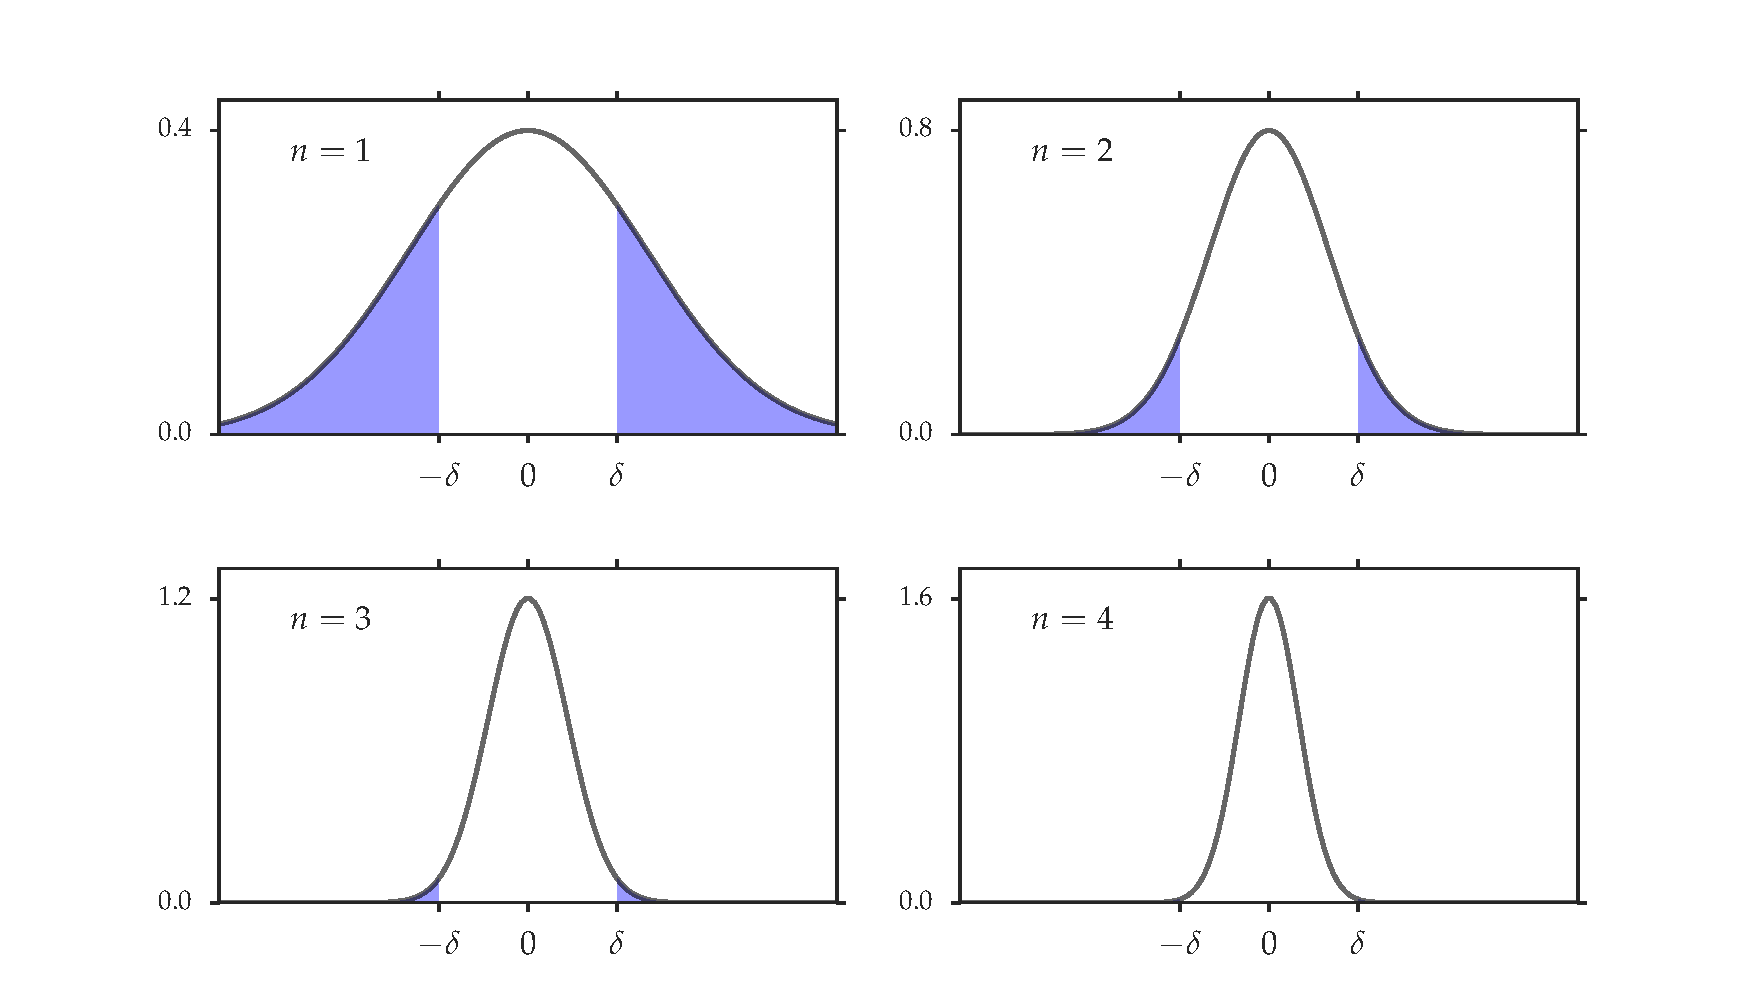
\includegraphics[trim={4em 4em 4em 4em}, clip]{conv_in_prob.pdf}}
    \caption{\label{f:conv_prob}  $\PP \{ |x_n | > \delta \} \to 0$ when
    $\lL(x_n) = \nN(0, 1/n)$}
    \end{figure}
    
\end{frame}

\begin{frame}

    \vspace{2em}
    \Fact\eqref{ET-fa:reconpro}
    The following statements are true:
    %
    \begin{enumerate}
        \item $\boldx_n \toprob \boldx \iff \| \boldx_n - \boldx \| \toprob
            0$
        \item $\boldx_n \toprob \boldx \implies g(\boldx_n) \toprob g(\boldx)$
            whenever $g$ is continuous at $\boldx$
        \item $\boldx_n \toprob \boldx$ and $\boldy_n \toprob \boldy$
            $\implies$ $\boldx_n + \boldy_n \toprob
            \boldx + \boldy$ and $\boldx_n^\T \boldy_n \toprob \boldx^\T
            \boldy$
        \item $\boldx_n \toprob \boldx$ and $\bolda_n \to \bolda$ $\implies$
            $\boldx_n + \bolda_n \toprob
            \boldx + \bolda$ and $\boldx_n^\T \bolda_n \toprob \boldx^\T
            \bolda$
        \item $\boldx_n \toprob \boldx$ $\iff$ $\bolda^\T \boldx_n \toprob \bolda^\T \boldx$ for any $\bolda \in \RR^K$
    \end{enumerate}
    
\end{frame}

\begin{frame}\frametitle{Convergence in mean square}
    
    \vspace{2em}
    The scalar sequence $\{x_n\}$ is said to converge to $x$ \navy{in mean square} 
    if
    %
    \begin{equation}
        \label{eq:cims}
        \EE (x_n - x)^2   \to 0 
        \quad \text{as} \quad n \to \infty
    \end{equation}
    %
    and we write \navy{$x_n \toms x$}
    
    \vspace{1em}
    Unlike convergence in probability, for
    convergence in mean square to be defined we require our variables to have
    finite second moments
    
\end{frame}

\begin{frame}
    
    \vspace{2em}
    \Fact\eqref{ET-fa:ffci}
    Let $\{x_n\}$ and $x$ have finite second moments and let $\alpha$ be any
    constant.  The following statements are true:
    %
    \begin{enumerate}
        \item $x_n \toms x \implies x_n \toprob x$.
        \item $x_n \toms \alpha$ $\iff$ $\EE x_n \to \alpha$ and $\var[x_n]
            \to 0$.
    \end{enumerate}
    
    \vspace{1em}
    Part 1. follows from Chebyshev's inequality --- $\PP\{|x| \geq \delta \} \leq \frac{\EE x^2}{\delta^2}$
    
    In particular, from monotonicity of $\PP$:
    %
    \begin{equation*}
        \PP\{|x_n - x| > \delta \} 
        \leq \PP\{|x_n - x| \geq \delta \} 
        \leq \frac{\EE (x_n - x)^2}{\delta^2}
    \end{equation*}
    %
\end{frame}

\begin{frame}

    \vspace{2em}
    Part 2. of the above is implied by:
    
    \Fact\eqref{ET-fa:dmse0}
        For any $x \in L_2$ and any constant $\alpha$ we have
        %
        \begin{equation}
            \label{eq:dmse0}
            \EE [ (x - \alpha)^2 ] = \var[x] + (\EE[x] - \alpha)^2
        \end{equation}
        
    Proof is an exercise. 
    

\end{frame}

\begin{frame}
    
    \vspace{2em}
    As a prelude to the Law of Large Numbers (LLN), let's consider the
    effects of averaging over independent random quantities
    
    Let 
    %
    \begin{itemize}
        \item $x_n$ be the payoff from holding one dollar of asset $n$,
        \item $\EE x_n = \mu$ and $\var[x_n] = \sigma^2$ for all $n$, and
        \item $\cov[x_j, x_k] = 0$ when $j \not= k$.
    \end{itemize}
    
    \vspace{1em}
    If we hold just asset 1, then the payoff is $x_1$, the expected payoff is $\mu$
    and the variance is $\sigma^2$
    
\end{frame}


\begin{frame}

    \vspace{2em}
    If we diversify by
    spreading one dollar evenly over $N$ of these assets, our payoff is
    %
    \begin{equation*}
        \bar x_N := \frac{1}{N} \sum_{n=1}^N x_n
    \end{equation*}
    
    \vspace{1em}
    The expected payoff is unchanged at 
    %
    \begin{equation*}
        \label{eq:meanub}
        \EE  \bar x_N 
            = \EE \left[ \frac{1}{N} \sum_{n=1}^N x_n \right]
            = \frac{1}{N} \sum_{n=1}^N \EE  x_n 
            = \mu
    \end{equation*}
    %
    
\end{frame}


\begin{frame}

    \vspace{2em}
    But the variance declines at rate $\frac{1}{N}$ because
    %
    \begin{align*}
        \EE [(\bar x_N - \mu)^2 ]  
        & = \EE \left\{ \left[ \frac{1}{N} \sum_{i=1}^N (x_i - \mu) \right]^2 \right\}
        \\
        & = \frac{1}{N^2} \sum_{i=1}^N \sum_{j=1}^N \EE (x_i - \mu)(x_j - \mu) 
        \\& = \frac{1}{N^2} \sum_{i=1}^N \EE (x_i - \mu)^2 
        = \frac{\sigma^2}{N} 
    \end{align*}
    
    The important equality here is the third one, which holds because of the zero
    covariance between assets
    
\end{frame}

\begin{frame}

    \vspace{2em}
    To summarize,
    %
    \begin{equation}
        \label{eq:sosm}
        \EE \bar x_N = \mu 
        \quad \text{and} \quad
        \var[ \bar x_N ] = \frac{\sigma^2}{N}
        \quad \text{for all } N
    \end{equation}
    %
    By taking $N \to
    \infty$ and combining \eqref{eq:sosm} with fact~\ref{ET-fa:ffci} above we obtain a proof of 
    the \navy{law of large numbers}:

    \vspace{1em}
    \Thm
        \eqref{ET-t:lln0}
        Let $\{x_n\}$ be {\sc iid} copies of $x$.  If $x$ is integrable, then
        %
        \begin{equation}
            \label{eq:lln0}
            \frac{1}{N} \sum_{n=1}^N x_n \toprob \EE x 
             \quad \text{ as } \quad N \to \infty
        \end{equation}
    
    
    We assumed finite second moment: see ET page 164 for references on proofs for the LLN without assumption on second moment

\end{frame}

\begin{frame}

    \vspace{2em}
    We can extend \eqref{eq:lln0} to 
    arbitrary functions of random variables and random vectors:
    
    \vspace{1em}
    If
    $\boldx$ is any random vector, $\{\boldx_n\}$ are {\sc iid} copies and
    $h \colon \RR^N \to \RR$ is any $\bB$-measurable function such that
    $h(\boldx)$ is integrable, then
    %
    \begin{equation*}
        \label{eq:lln0g}
        \frac{1}{N} \sum_{n=1}^N h(\boldx_n) \toprob \EE  h(\boldx) 
             \quad \text{ as } \quad N \to \infty
    \end{equation*}
    
    Proof follows from Theorem \eqref{ET-t:lln0} (exercise, or see page 164 of ET)
    
\end{frame}

\begin{frame}

    \vspace{2em}
    The law of large numbers applies to probabilities as well as
    expectations
    
    \vspace{1em}
    Fix $B \subset \bB(\RR^N)$, let $h(\bolds) = \1_B(\bolds) = \1\{\bolds \in B\}$,
    we have
    %
    \begin{equation*}
        \EE h(\boldx)  = \EE \1\{\boldx \in B\}  = \PP \{\boldx \in B\} 
    \end{equation*}
    %
    Combine this equality with the LLN, 
    if $\{\boldx_n\}$ is {\sc iid} with distribution $P$, then
    %
    \begin{equation*}
        \label{eq:lln0lg}
        \frac{1}{N} \sum_{n=1}^N \1\{\boldx_n \in B\} \toprob P(B)
    \end{equation*}
    %
    The fraction of the sample that falls in $B$
    converges to the probability that the distribution assigns to $B$
    
\end{frame}

\begin{frame}

    \vspace{2em}
    To illustrate the law of large numbers, consider flipping a coin until
    10 heads have occurred
    
    \begin{itemize}
    \item probability of heads is
    0.4
    \end{itemize}
    
    \vspace{1em}
    Let $x$ be the number of tails observed in the process
    \begin{itemize}
        \item random variable is known to have the \navy{negative binomial
    distribution} with $\EE x =15$
    \end{itemize}
    
    The LLN predicts that 
    if we simulate a large number of observations of $x$ and take the average,
    we get a value close to 15

\end{frame}

\begin{frame}[fragile]

    \vspace{2em}
    Julia code to illustrate LLN:
    \begin{juliacode}
num_reps = 10^6
outcomes = Array(Float64, num_reps)

for i in 1:num_reps
    num_tails = num_heads = 0
    while num_heads < 10
        b = rand()
        num_heads = num_heads + (b < 0.4)   
        num_tails = num_tails + (b >= 0.4) 
    end
    outcomes[i] = num_tails
end

println(mean(outcomes))
    \end{juliacode}

\end{frame}

\begin{frame}

    \vspace{2em}
    What happens when the finite first
    moment condition in the LLN is not enforced?
    
\end{frame}

\begin{frame}

    \vspace{2em}
    \begin{figure}
    \centering
    \scalebox{.44}{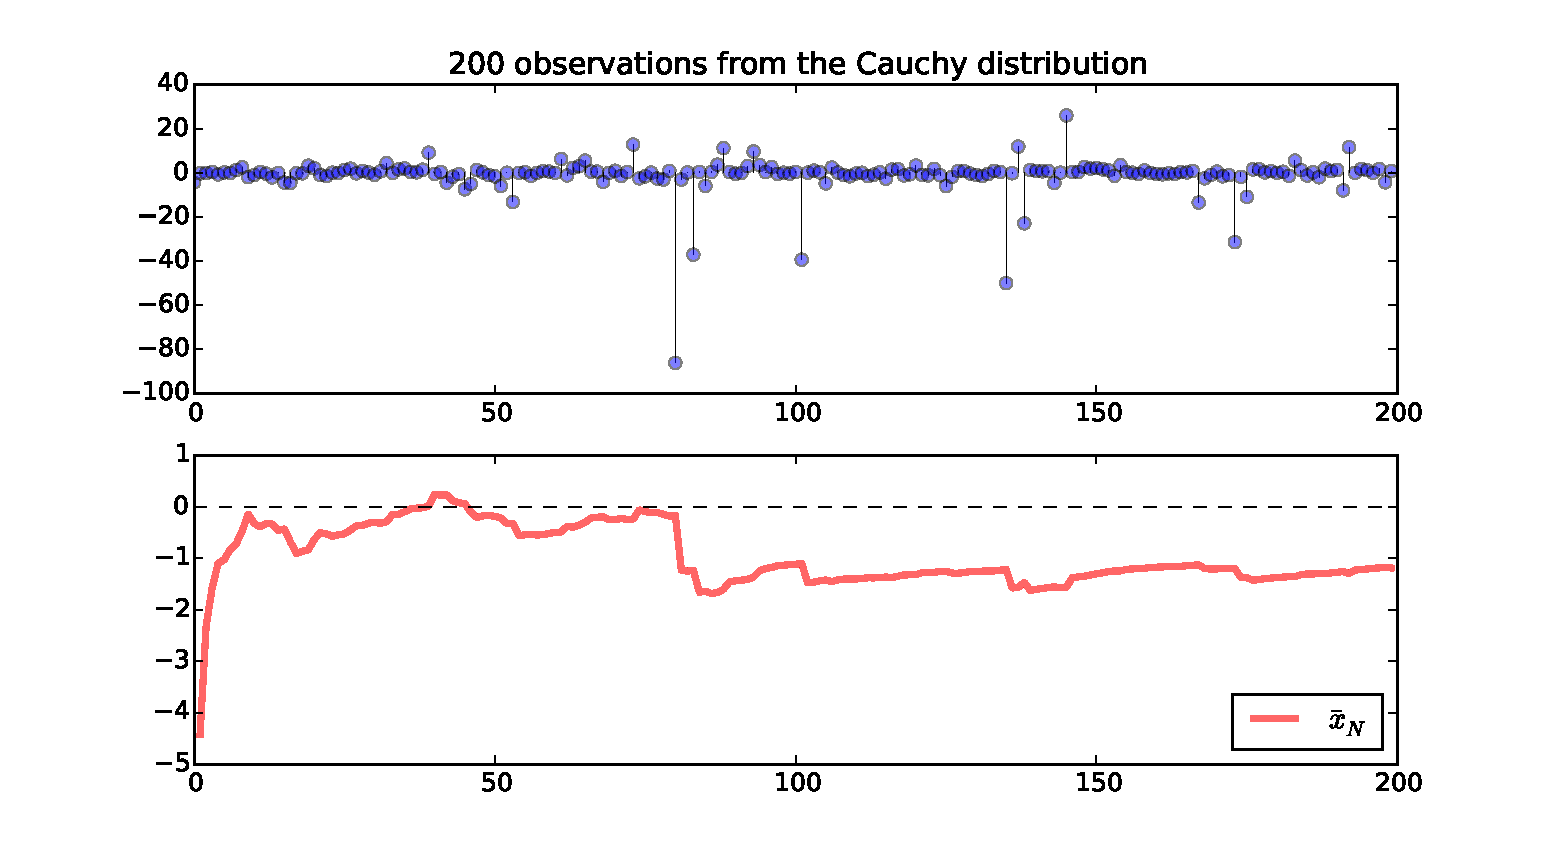
\includegraphics[trim={5em 5em 5em 5em}, clip]{cauchy_samples.pdf}}
    \caption{\label{f:cauchy_samples} Samples from the Cauchy distribution and sample mean}
    
\end{figure}

\end{frame}

\begin{frame}\frametitle{Convergence in Distribution}

    \vspace{2em}
    The common notion of convergence of distributions, which is
    called weak convergence, requires $P_n(B) \to P(B)$ for all
    ``continuity sets" in $\RR^K$
    
    \vspace{1em}
    Equivalently: $\{P_n\}$ \navy{converges weakly} to $P$ if
    %
    \begin{align*}
        \int h(\bolds) P_n(\diff \bolds) \to \int h(\bolds) P(\diff \bolds)
        \quad 
        \\ \text{$\forall$ continuous bounded $h \colon \RR^K \to \RR$}
    \end{align*}
    %
    and we write \navy{$P_n \tow P$}
    
\end{frame}

\begin{frame}

    \vspace{2em}
    \Fact(6.1.4)
    Let $F_n$ be the {\sc cdf} of $P_n$ and let $F$ be the {\sc cdf} of $P$.
    In the univariate case ($K=1$) we have 
    
    \begin{align*}
        P_n \tow P 
        \quad \iff \quad
        F_n(s) \to F(s) 
        \\ \; \text{ for all $s$ at which $F$ is continuous}
    \end{align*}

    \vspace{1em}
    \Eg
        It can be shown that the $t$-distribution with $k$ degrees of freedom
        converges weakly to the standard normal distribution as $k \to \infty$
    
\end{frame}

    \vspace{2em}
    \begin{frame}
        \begin{figure}
       \begin{center}
        \scalebox{.4}{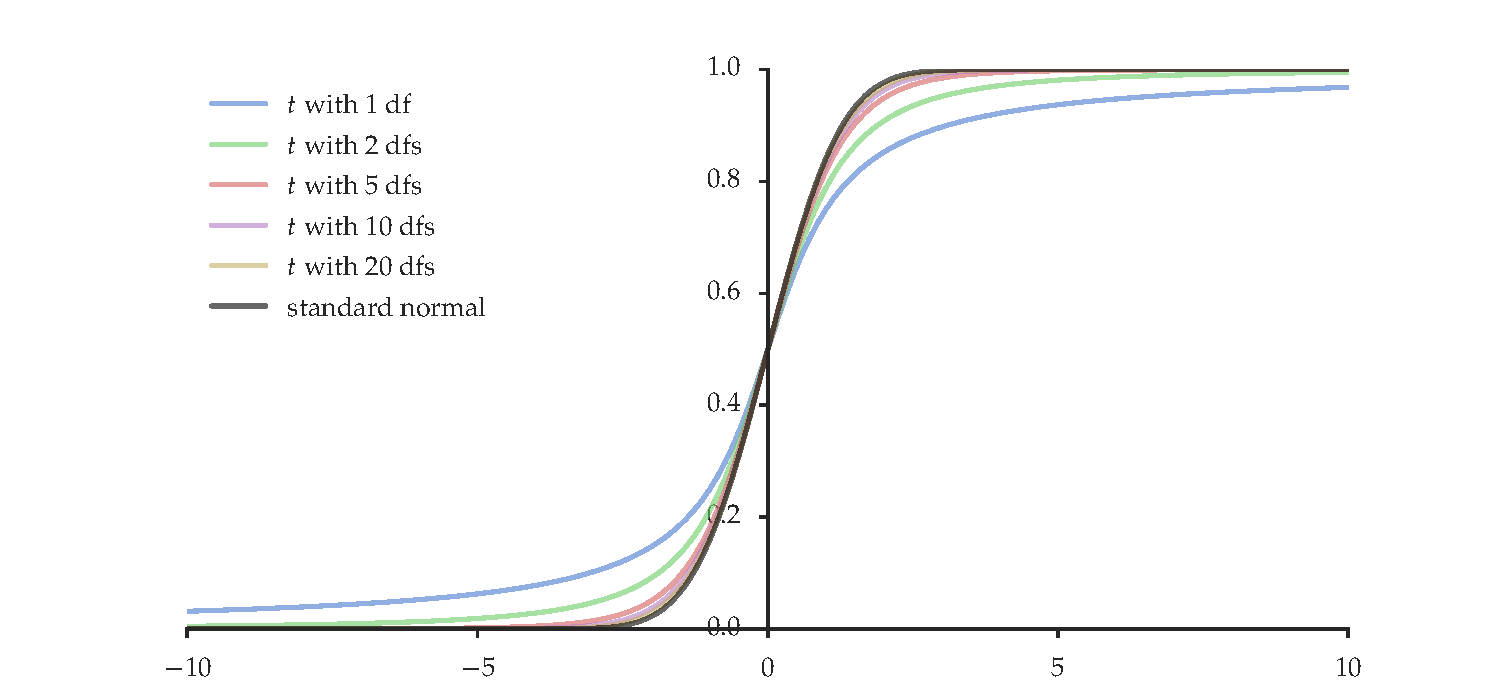
\includegraphics{t_to_norm.pdf}}
        \caption{\label{f:t_to_norm} $t$-Distribution with $k$ df converges to $\nN(0,1)$ as $k \to \infty$}
       \end{center}
    \end{figure}
      
\end{frame}

\begin{frame}

    \vspace{2em}
    \Fact\eqref{ET-fa:cdicd}
    Let $\{P_n\}$ and $P$ be absolutely continuous probability measures on
    $\RR^K$, with densities $p_n$ and $p$
    
    If $p_n(\bolds) \to p(\bolds)$ for all
    $\bolds \in \RR^K$, then $P_n \tow P$

\end{frame}

\begin{frame}

    \vspace{2em}
    Let $\{\boldx_n\}$ and $\boldx$ be random vectors
    
    We say $\boldx_n \to \boldx$ \navy{in
    distribution} if their respective distributions converge weakly
    
    The
    convergence is symbolized by $\boldx_n \tod \boldx$
    
    Thus
    %
    \begin{equation*}
        \boldx_n \tod \boldx
        \; \iff \;
        \lL(\boldx_n) \tow \lL(\boldx)
    \end{equation*}
    %
    Equivalent to:
    %
    \begin{equation*}
        \EE[ h(\boldx_n)]  \to \EE[ h(\boldx) ]
        \quad 
        \text{for all continuous bounded $h \colon \RR^K \to \RR$}
    \end{equation*}
    %
    (Why?)
    
\end{frame}

\begin{frame}

    \vspace{2em}
    \Fact\eqref{ET-fa:cmtetc}
    The following statements are true:
    %
    \begin{enumerate}
        \item If $g \colon \RR^K \to \RR^J$ is continuous and
            $\boldx_n \tod \boldx$, then $g(\boldx_n) \tod g(\boldx)$.
        \item If $\bolda^\T \boldx_n \tod \bolda^\T \boldx$ for any $\bolda \in \RR^K$,
            then $\boldx_n \tod \boldx$.
        \item $\boldx_n \toprob \boldx \implies \boldx_n \tod \boldx$.
        \item If $\bolda$ is a constant vector and $\boldx_n \tod \bolda$,
            then $\boldx_n \toprob \bolda$
    \end{enumerate}
    
    Part 1. called the \navy{continuous mapping
    theorem}
    
    Part 2.  called the 
    Cram\'er--Wold theorem, or the \navy{Cram\'er--Wold device}
    
\end{frame}

\begin{frame}

    \vspace{2em}
    \Fact\eqref{ET-fa:slut}
        If $\alpha$ is constant, $x_n \toprob \alpha$ and $y_n \tod y$, then
            $x_n + y_n \tod \alpha + y$ and $x_n y_n \tod \alpha y$
    
    \vspace{1em}
    An immediate but useful consequence is that 
    
    \Fact\eqref{ET-fa:sluti}
        $x_n \toprob 0$ and $y_n \tod y$ $\implies$ $x_n y_n \toprob 0$

\end{frame}


\begin{frame}\frametitle{The Central Limit Theorem}

    \vspace{2em}
    The \navy{central limit theorem} 
    is among the most striking and important results in all of
    mathematics
    
    \vspace{1em}
    \Thm\eqref{ET-t:clt0}
        Let $x$ have finite second
        moment and let $\{x_n\}$ be {\sc iid} copies of $x$.  If
        $\mu := \EE x$ and $\sigma^2 := \var x$, then
        %
        \begin{equation*}
            \label{eq:clt0}
            \sqrt{N} (\bar x_N - \mu) 
            \tod \nN(0, \sigma^2)
             \quad \text{ as } \quad
             N \to \infty
        \end{equation*}
        
\end{frame}

\begin{frame}

    \vspace{2em}
    On one hand, $(\bar x_N - \mu) \toprob 0$ by the LLN; 
    on the other hand, $\sqrt{N} \to \infty$
    
    If we take the product, these two
    competing terms just balance
    
    \vspace{1em}
    The distribution of the product
    approaches a zero-mean Gaussian as $N \to \infty$, regardless of the
    distribution of $x$
    
\end{frame}

\begin{frame}

    \vspace{2em}
    Consider simulating the CLT
    
    Let $Q_N :=$ the distribution of $\sqrt{N} (\bar x_N - \mu)$
    for $N=1,\ldots,5$
    
    Initial distribution $Q=Q_1$ is multi-modal,
    constructed as a convex combination of three beta distributions
    
\end{frame}

\begin{frame}

    \vspace{2em}
    \begin{figure}
    \centering
    \scalebox{.46}{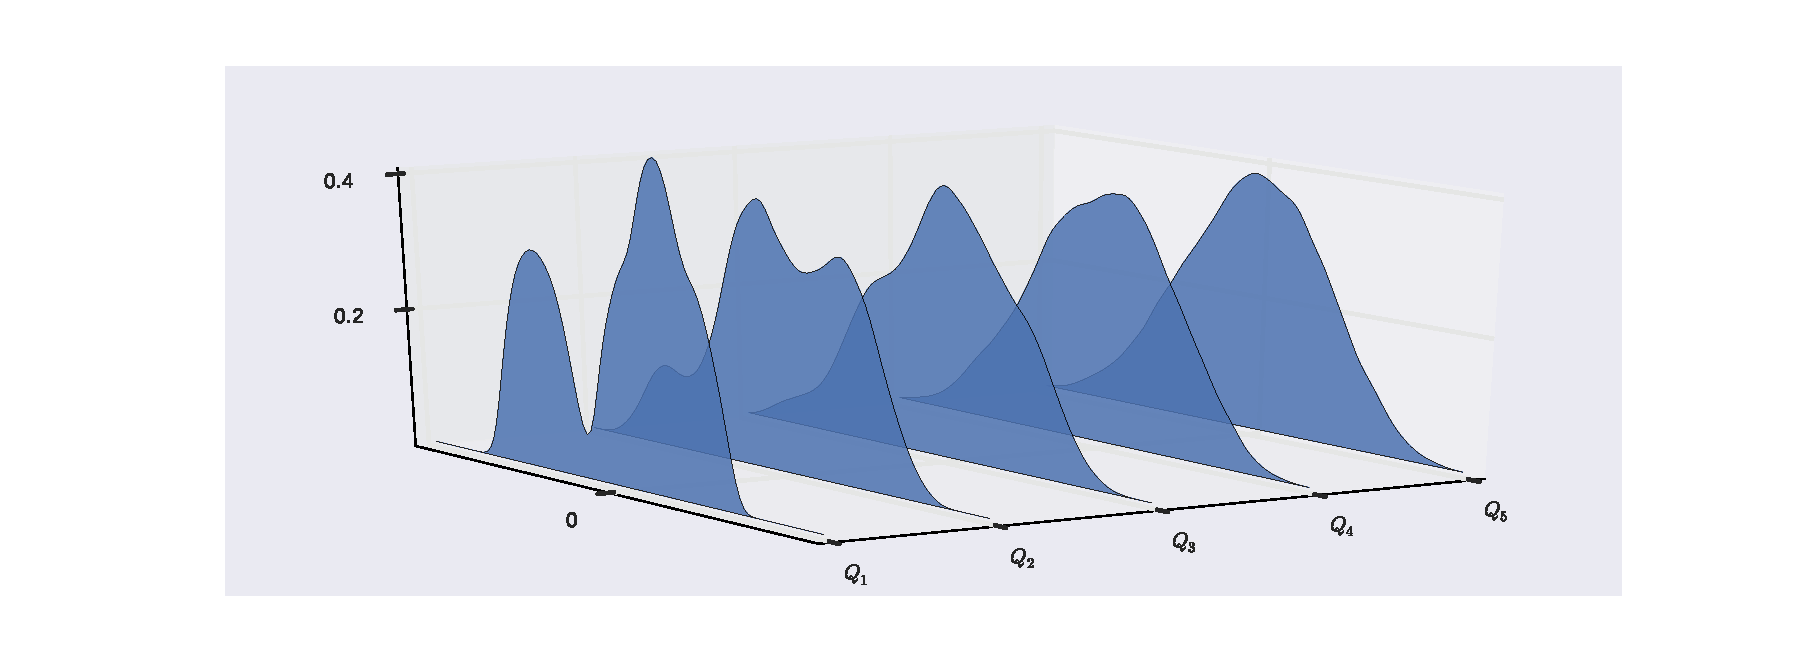
\includegraphics[trim={5em 2em 10em 2em}, clip, center]{clt3d_2.pdf}}
    \caption{\label{f:clt3d} CLT in action, starting from a beta mixture}
    \end{figure}
    
\end{frame}

\begin{frame}
    
    \vspace{2em}
    Another common statement of the central limit theorem:  if all the conditions of the CLT are satisfied, then

    \begin{equation*}
        \label{eq:clt1}
        z_N := \sqrt{N} \left\{ \frac{\bar x_N - \mu}{\sigma}  \right\}
        \tod \nN(0,1)
        \quad \text{ as } \quad
        N \to \infty
    \end{equation*}
    
\end{frame}

\begin{frame}[fragile]

    \vspace{2em}
    Python code to illustrate CLT:
    \begin{pythoncode}
import numpy as np
import scipy.stats as st

num_reps = 5000
outcomes = np.empty(num_reps)
N, k = 1000, 5     # k = degrees of freedom
chi = st.chi2(k)

for i in range(num_reps):
    xvec = chi.rvs(N)
    outcomes[i] = np.sqrt(N / (2 * k))\
                  *(xvec.mean() - k) 

    \end{pythoncode}
    
\end{frame}

\begin{frame}

    \vspace{2em}
    The listing generates 5,000 observations of
    
    \begin{equation*}
    z_N := \sqrt{N} \left\{ \frac{\bar x_N - \mu}{\sigma}  \right\}
    \tod \nN(0,1)
    \quad \text{ as } \quad
    N \to \infty
    \end{equation*}
    
    Each $x_n$ is $\chi^2(5)$
    \begin{itemize}
        \item mean of this distribution is 5, and the variance is $2
    \times 5 = 10$
    \end{itemize}
    
    \vspace{1em}
    The observations of $z_N$ are stored in the vector
    \mintinline{python}{outcomes}
    
\end{frame}

\begin{frame}

    \begin{figure}
       \begin{center}
        \scalebox{.44}{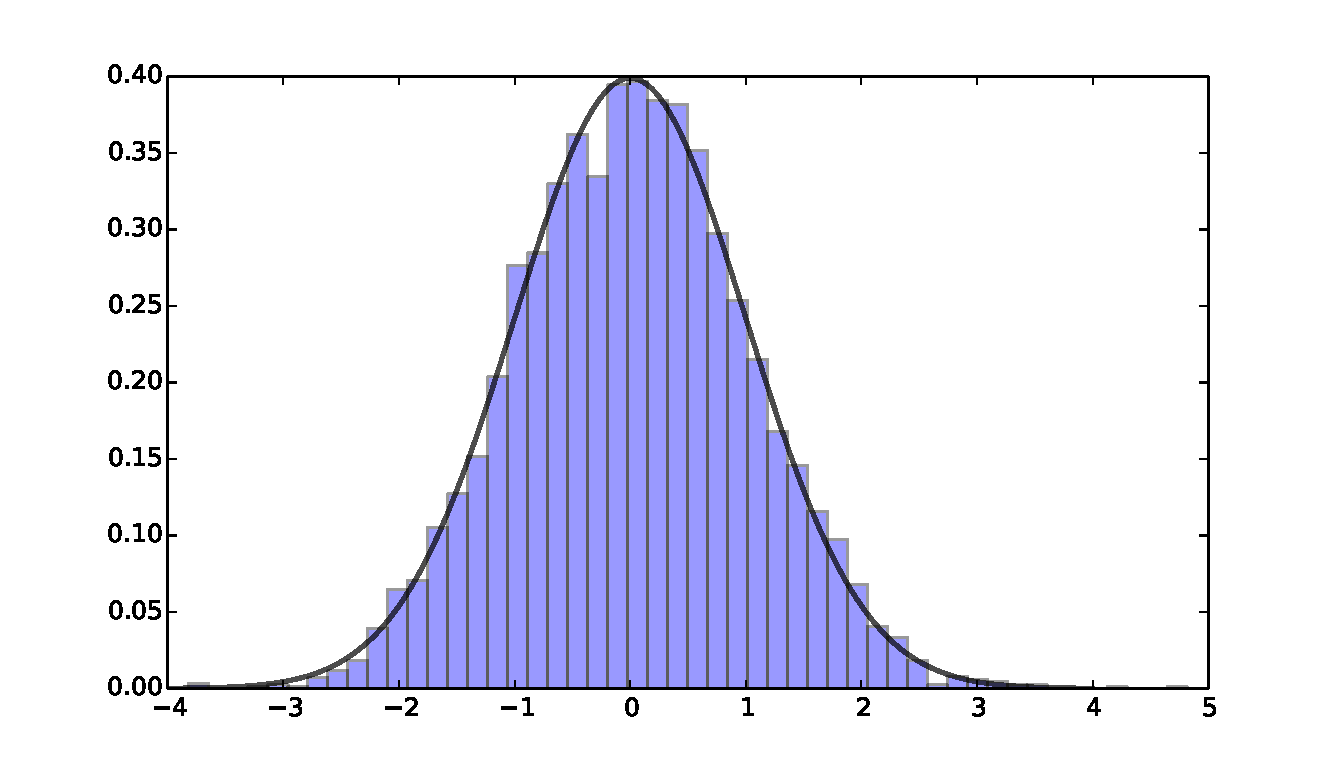
\includegraphics{illus_clt.pdf}}
        \caption{\label{f:illus_clt} Observations of $z_N$ in \eqref{eq:clt1} when the underlying distribution is $\chi^2(5)$}
       \end{center}
    \end{figure}

\end{frame}

\section{Extensions of CLT and LLN}

\begin{frame}\frametitle{Convergence of Random Matrices}

    \vspace{2em}
    Let $\{\boldX_n\}_{n=1}^{\infty}$ be a sequence of random
    $N \times K$ matrices.  We say that $\boldX_n$ converges to a random $N
    \times K$ matrix $\boldX$ \navy{in probability} and write $\boldX_n \toprob
    \boldX$ if 
    %
    \begin{equation*}
        \| \boldX_n - \boldX \| \toprob 0
        \quad \text{as} \quad n \to \infty
    \end{equation*}
    %
    where $\| \cdot \|$ is the matrix norm defined in \S\ref{ET-ss:mn}
    
\end{frame}

\begin{frame}

    \vspace{2em}
    \Fact\eqref{ET-fa:cmtetcv1}
    Assuming conformability, the following statements are true:
    %
    \begin{enumerate}
        \item If $\boldX_n \toprob \boldX$ and $\boldX_n$ and $\boldX$ are 
            nonsingular, then $\boldX_n^{-1} \toprob \boldX^{-1}$.
        \item If $\boldX_n \toprob \boldX$ and $\boldY_n \toprob \boldY$, then
            %
            \begin{equation*}
                \boldX_n + \boldY_n \toprob \boldX + \boldY,
                \quad
                \boldX_n \boldY_n \toprob \boldX \boldY,
                \quad \text{and} \quad
                \boldY_n \boldX_n \toprob \boldY \boldX
            \end{equation*}
            %
        \item If $\boldX_n \toprob \boldX$ and $\boldA_n \to \boldA$, then
            %
            \begin{equation*}
                \boldX_n + \boldA_n \toprob \boldX + \boldA,
                \quad
                \boldX_n \boldA_n \toprob \boldX \boldA,
                \quad \text{and} \quad
                \boldA_n \boldX_n \toprob \boldA \boldX
            \end{equation*}
     \seti        %
    \end{enumerate}
    
\end{frame}

\begin{frame}

    \vspace{2em}
    \begin{enumerate}
        \conti
        \item $\boldX_n \toprob \boldX$ if and only if $\boldX_n \bolda \toprob
        \boldX \bolda$ for any conformable vector $\bolda$
        \item $\bolda^\T \boldX_n \bolda \toprob \bolda^\T \boldX \bolda$
             whenever $\bolda$ is a conformable constant vector and 
             $\boldX_n \toprob \boldX$
    \end{enumerate}
    
\end{frame}

\begin{frame}

    \vspace{2em}
    In econometrics we often use the vector version of Slutsky's theorem:

    \vspace{1em}
    \Fact\eqref{ET-fa:cmtetcv2}
        Let $\boldx_n$ and $\boldx$ be random vectors in $\RR^K$, let 
        $\boldY_n$ be random matrices, and let $\boldC$ be a constant matrix.
        Assuming conformability, we have
        %
        \begin{align*}
            \boldY_n \toprob \boldC \text{ and } \boldx_n \tod \boldx
            \quad \implies \quad
                \boldY_n \boldx_n \tod \boldC \boldx
                \quad \\ \text{and} \quad
                \boldY_n + \boldx_n \tod \boldC + \boldx
        \end{align*}

\end{frame}

\begin{frame}

    \vspace{2em}
    The scalar LLN and CLT extend to the vector case:
    
    \Thm\eqref{ET-t:vllnclt}
        Let $\boldx$ be a random vector in $\RR^K$ and let $\{\boldx_n\}$ be {\sc
        iid} copies of $\boldx$.  If $\boldmu := \EE \boldx$ is finite, then
        %
        \begin{equation}
            \label{eq:vlln}
            \bar \boldx_N :=
            \frac{1}{N} \sum_{n=1}^N \boldx_n \toprob \boldmu
             \quad \text{ as } \quad N \to \infty
        \end{equation}
        %
        If, in addition, $\EE \|\boldx\|^2 < \infty$, then
        %
        \begin{equation}
            \label{eq:vclt}
            \sqrt{N} \left( \bar \boldx_N - \boldmu \right)
            \tod \nN(\boldzero, \Sigma)
            \quad \text{where } \;
            \Sigma := \var \boldx
        \end{equation}
    %
    Here $\frac{1}{N} \sum_{n=1}^N \boldx_n$ should
    be understood in terms of vector addition and scalar multiplication

\end{frame}

\begin{frame}

    \vspace{2em}
    \begin{figure}
       \begin{center}
        \scalebox{.7}{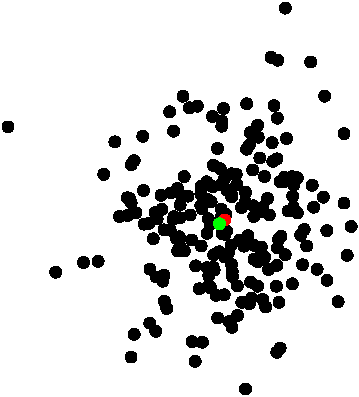
\includegraphics{vector_mean.pdf}}
        \caption{\label{f:vector_mean} LLN, vector case}
       \end{center}
    \end{figure}

\end{frame}

\begin{frame}

    \vspace{2em}
    Vector LLN in theorem~\ref{ET-t:vllnclt} follows from the scalar LLN 
    
    \begin{itemize}
        \item let $\boldx_n$ be $\{\boldx_n\}$ be {\sc
        iid} copies of $\boldx$
        \item let $\bolda$ be any
    constant vector in $\RR^K$
        \item define $y_n := \bolda^\T \boldx_n$
        \item define $y := \bolda^\T \boldx$
    \end{itemize}
    
    The sequence $\{y_n\}$ is {\sc iid}
    (see fact~\ref{ET-fa:rviifi} on page~\pageref{ET-fa:rviifi})
    with the same distribution as $y$
    
    By the scalar LLN
    %
    \begin{equation*}
        \frac{1}{N} \sum_{n=1}^N y_n \toprob \EE y 
        = \EE[\bolda^\T \boldx]
        = \bolda^\T\EE[ \boldx]
        = \bolda^\T \boldmu
    \end{equation*}
    
\end{frame}

\begin{frame}

    \vspace{2em}
    At the same time:
    %
    \begin{equation*}
        \frac{1}{N} \sum_{n=1}^N y_n 
        = \frac{1}{N} \sum_{n=1}^N \bolda^\T \boldx_n 
        = \bolda^\T \left[ \frac{1}{N} \sum_{n=1}^N  \boldx_n \right]
        = \bolda^\T \bar \boldx_N
    \end{equation*}
    
    \vspace{2em}
    Thus 
    %
    \begin{equation*}
       \bolda^\T \bar \boldx_N \toprob \bolda^\T \boldmu \; \text{ for any }\;
       \bolda \in \RR^K
    \end{equation*}
    %
   
    The claim $\bar \boldx_N \toprob \boldmu$ now follows (recall fact 6.1.1 above)
    
\end{frame}

\begin{frame}

    \vspace{2em}
    \Fact\eqref{ET-fa:llnmat}
    Let $\boldX$ be a random matrix and let $\{\boldX_n\}$ be
    {\sc iid} copies of $\boldX$.  If $\EE \| \boldX \|< \infty$, 
    then
    %
    \begin{equation}
        \frac{1}{N} \sum_{n=1}^N \boldX_n \toprob \EE  \boldX 
         \quad \text{ as } \quad N \to \infty
    \end{equation}
    
    
    \Prf
    Since $\boldX_n \bolda$ is a vector with expectation $\EE [ \boldX ] \bolda $, the following
    %
    $$\frac{1}{N} \sum_{n=1}^N \boldX_n \bolda \toprob \EE [ \boldX] \bolda $$
    %
    for any conformable vector $\bolda$, is immediate from the vector LLN (theorem~\ref{ET-t:vllnclt})


\end{frame}

\begin{frame}

    \vspace{2em}
    The proof for Fact \ref{ET-fa:llnmat} is then complete by recalling the following from fact \ref{ET-fa:reconpro}
    
    \[\boldx_n \toprob \boldx \quad \iff \quad \bolda^\T \boldx_n \toprob \bolda^\T \boldx \quad \text{for any}\quad \bolda \in \RR^K\]
    
\end{frame}

\begin{frame}\frametitle{The Delta Method}

    \vspace{2em}
    We showed the asymptotic normality result in the central limit theorem is preserved
    under linear transformations (fact~\ref{ET-fa:cmtetcv2})
    
    The result also holds for functions that are locally
    almost linear --- for differentiable functions
    
    \vspace{1em}
    \Thm\eqref{ET-t:dm}
    Let $g \colon \RR^K \to \RR$, let $\boldtheta$ be a point in the domain
    of $g$, and let $\{\boldt_n\}$ be a sequence of
    random vectors in $\RR^K$. If
    %
    \begin{enumerate}
        \item $\sqrt{n} (\boldt_n - \boldtheta) \tod \nN(0, \boldSigma)$ for
            some positive definite $\boldSigma$ and
        \item $\nabla g(\boldtheta)$ exists, is continuous, and each element is nonzero
    \end{enumerate}
    %
    then
    %
    \begin{equation}
        \label{eq:dmmv}
        \sqrt{n} \{ g(\boldt_n) - g(\boldtheta) \}
        \tod \nN(0, \nabla g(\boldtheta)^\T \boldSigma \nabla g(\boldtheta))
         \quad \text{ as } \quad
         n \to \infty
    \end{equation}
    
\end{frame}



\begin{frame}

    \vspace{2em}
    The term $\nabla g(\boldtheta)$ is the \navy{gradient vector}
    of $g$ at $\boldtheta$:
    %
    \begin{equation*}
        \nabla g(\boldtheta)
        := 
        \begin{pmatrix}
             g'_1(\boldtheta)
             \\
             \vdots
             \\
             g'_K(\boldtheta)
        \end{pmatrix}
        \quad \text{where} \quad
        g'_k (\boldtheta) := \frac{\partial g(\boldtheta)} {\partial \theta_k}
    \end{equation*}
    
    \vspace{1em}
    In the scalar case, \eqref{eq:dmmv} translates to     
    %
    \begin{equation*}
        \label{eq:dm0}
        \sqrt{n} \{ g(t_n) - g(\theta) \}
        \tod \nN(0, g'(\theta)^2 \sigma^2)
         \quad \text{ as } \quad
         n \to \infty
    \end{equation*}
    
\end{frame}

\end{document}
